\chapter{Mengenal Python dan Anaconda}
Tujuan pembelajaran pada pertemuan pertama antara lain:
\begin{enumerate}
\item
Mengerti sejarah python, perkembangan dan penggunaan python di perusahaan
\item
Memahami tahapan instalasi python dan anaconda
\item
Memahami cara penggunaan spyder
\end{enumerate}
Tugas dengan cara dikumpulkan dengan pull request ke github dengan menggunakan format latex pada repo yang dibuat oleh asisten IRC.

\section{Teori}
Praktek teori penunjang yang dikerjakan :
\begin{enumerate}
\item
Buat Resume Sejarah Python, perbedaan python 2 dan 3, dengan bahasa yang mudah dipahami dan dimengerti. Buatan sendiri bebas plagiat(10)

jawaban:
Phyton merupakan bahasa pemrograman yang di kembangkan oleh Guido van Rossum pada tahun 1990 di CWI,Amsterdam sebagai kelanjutan dari bahasa pemrograman ABC.dan merupakan bahasa pemrograman yang interpratif multiguna dengan filosfi perancangan yang berfokus pada tingkat keterbacan kode.
Pengembangan phyton saat ini terus dilakukan oleh pemrogram yang dipimpin oleh guido dan phyton software foundation .organisasi ini merupakan pemegan hak cipta sejak versi 2.1  dan saat ini phyton sudah mencapai versi 2.6.1 dan versi 3.0
•	Perbedan phyton 2 dan 3
Phyton 2 di publikasikan pada pada tahun 2000 sedangkan phyton 3 di pulikasikan pada tahun 2008.perbedaan nya itu yakni phton 2 dinilai lebih transparan dalam pengembangan software daripada versi sebelum nya dan phyton 2 dilengkapi dengan berbagai fitur programatikal seperti cycle detecting gabage colector untuk manajemen memori ,sedangkan phyton 3  merupakan pengembangan dari phyton sebelumya dan masih dikembangkan sampai sekarang.dan pyton 3 sendiri memiliki banyak perubahan dan fokus pada phyton 3 itu sendiri melakukan perapian pada codebase dan redundancy dan juga memasukan statement print ke dalam built  in  function 


\item
Buat Resume Implementasi dan penggunaan Python di perusahaan dunia, bahasa yang mudah dipahami(10)


jawaban:
youtube adalah contoh platform yang telah memanfaatkan Python dalam analisis data. terlihat pada bagaimana youtube merekomendasikan video seperti ketika anda mencari video musik yang sering anda cari di aplikasi nya dan youtube akan merekomendasikan apa yang sering anda cari di youtube .Berikut ini adalah beberapa poin penting tentang penggunaan Python dalam analisis data youtube:
Tim youtube memanfaatkan analitis. Mereka memanfaatkan Luigi, modul dari Python, yang disinkronisasi dengan Hadoop, sebuah framework berbasis Java yang memungkinkan pemrosesan data dengan ukuran sangat besar.


\end{enumerate}

\section{Instalasi}
Melakukan instalasi python dan anaconda versi 3 serta uji coba spyder. Dengan menggunakan bahasa yang mudah dimengerti dan bebas plagiat. 
Dan wajib skrinsut dari komputer sendiri.
\begin{enumerate}
\item
Instalasi python 3 (5)
jawaban:

a.	Jalankan instalasi terlebih dahulu dengan cara run adminisrator
    

    \begin{figure}
\begin{center} 
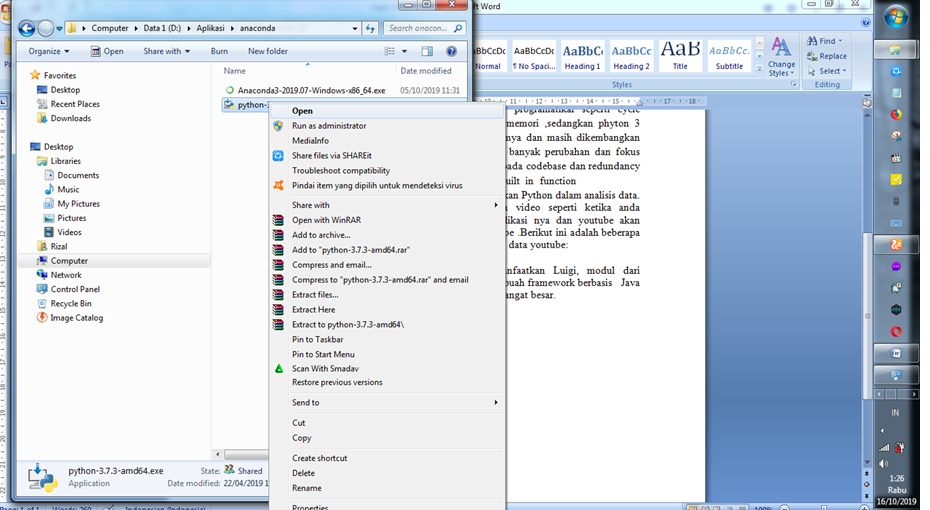
\includegraphics[scale=0.4]{src/soal1phyton1.PNG} 
\caption{gambar} 
\label{unhas} 
\end{center} 
\end{figure}

b. 	Pilih instal now

\begin{figure}
\begin{center} 
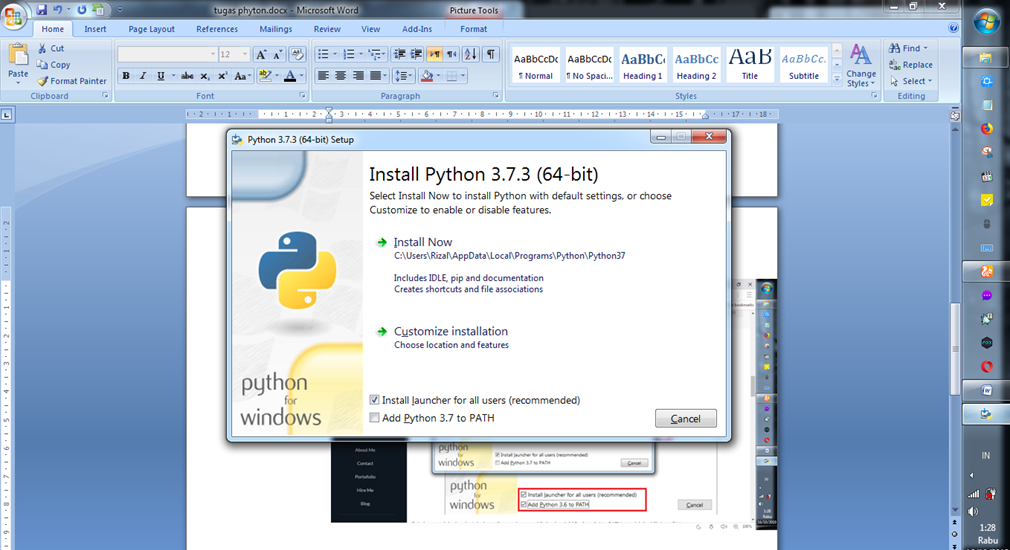
\includegraphics[scale=0.4]{src/soal1phyton2.PNG} 
\caption{gambar} 
\label{unhas} 
\end{center} 
\end{figure}

c.	Tunggu progress hingga selesai

\begin{figure}
\begin{center} 
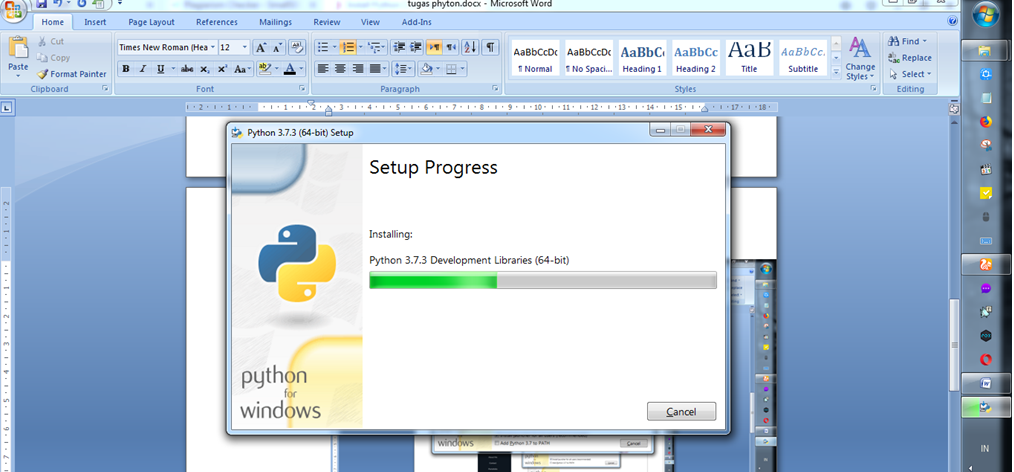
\includegraphics[scale=0.4]{src/soal1phyton3.PNG} 
\caption{gambar} 
\label{unhas} 
\end{center} 
\end{figure}

d.	Instalasi selesai close saja

\begin{figure}
\begin{center} 
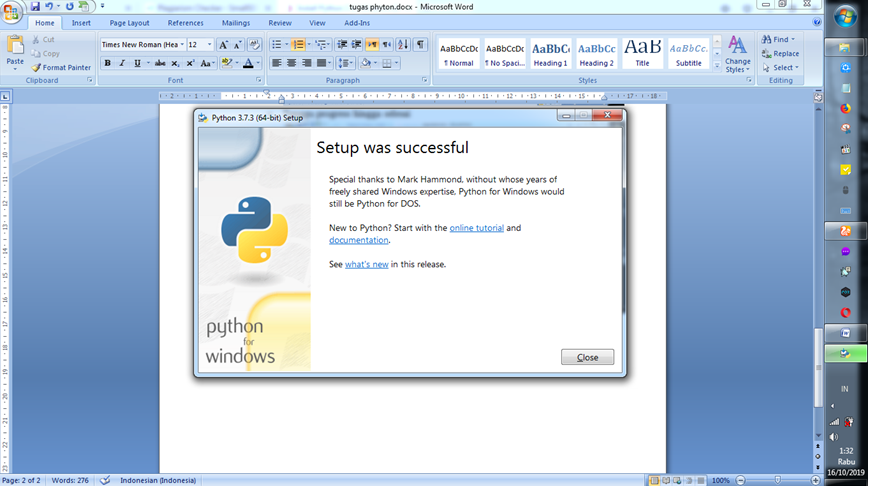
\includegraphics[scale=0.4]{src/soal1phyton4.PNG} 
\caption{gambar} 
\label{unhas} 
\end{center} 
\end{figure}

e.	Tampilan phyton 3

\begin{figure}
\begin{center} 
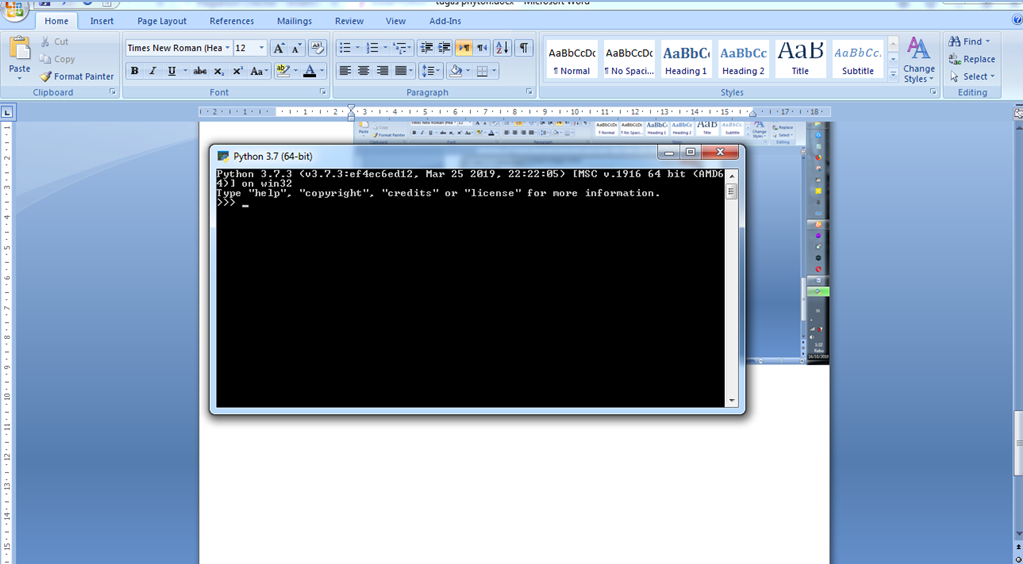
\includegraphics[scale=0.4]{src/soal1phyton5.PNG} 
\caption{gambar} 
\label{unhas} 
\end{center} 
\end{figure}

\item

 


instalasi pip(5)

jawaban:

a.	Download pip di instalasi dan klik kanan pada tulisan get.pp.py dan pilih link as dan pilih tempat penyimpanan anda

\begin{figure}
\begin{center} 
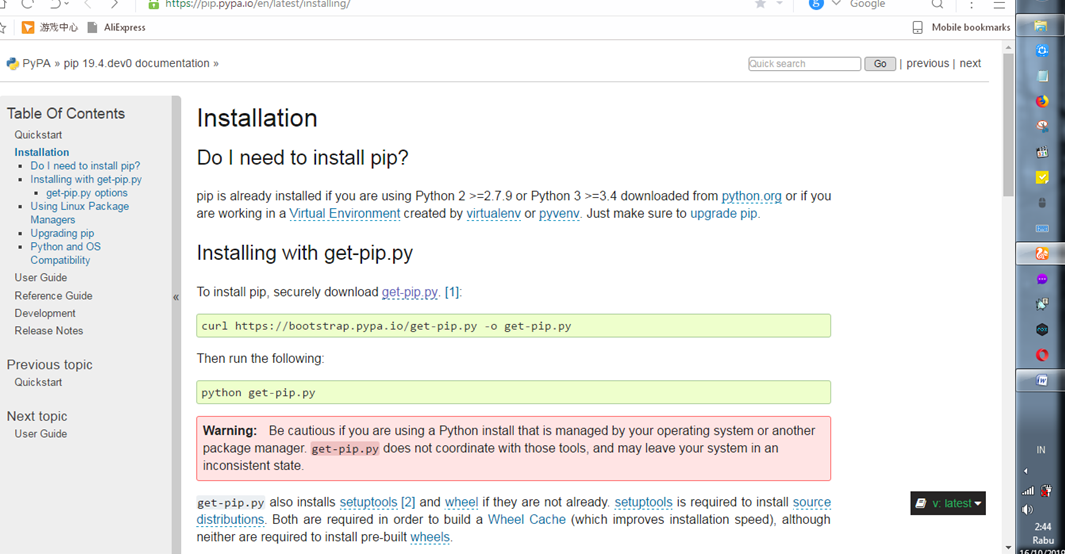
\includegraphics[scale=0.4]{src/soal2phyton1.PNG} 
\caption{gambar} 
\label{unhas} 
\end{center} 
\end{figure}

b.	Setelah di download file buka file anda tadi yang berformat phyton

\begin{figure}
\begin{center} 
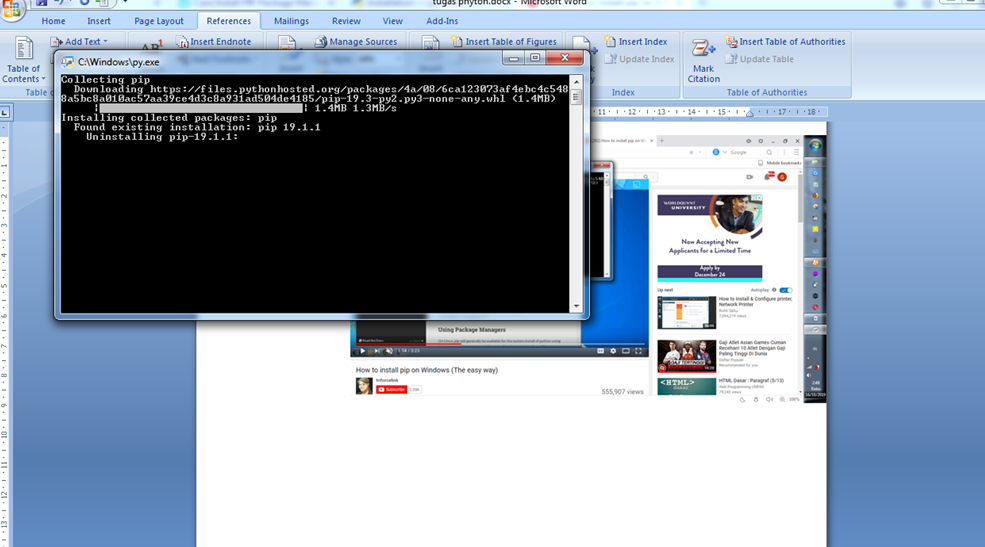
\includegraphics[scale=0.4]{src/soal2phyton2.PNG} 
\caption{gambar} 
\label{unhas} 
\end{center} 
\end{figure}

c.setelah itu instalasi akan selesai sendiri dan akan langsung selesai dan pip telah di instal di python dan masuk ke cmd dan tulis pip install request

\item
cara setting environment (5)

jawaban:
a.	Masuk ke control panel,system and security,system
    \begin{figure}
\begin{center} 
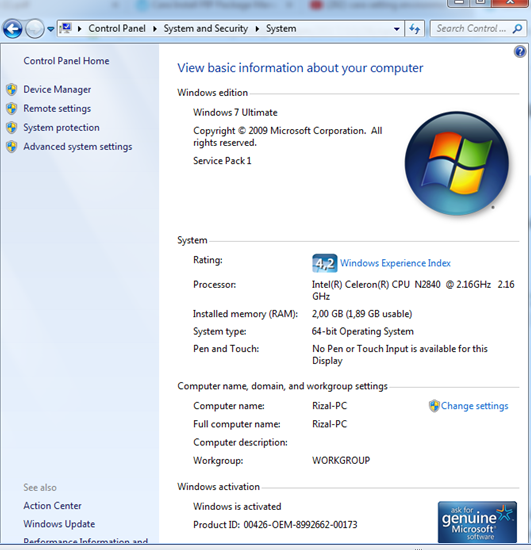
\includegraphics[scale=0.4]{src/soal3phyton1.PNG} 
\caption{gambar} 
\label{unhas} 
\end{center} 
\end{figure}

b.	Klik advanced system setting di tables advance dan pilih environtment tables
    \begin{figure}
\begin{center} 
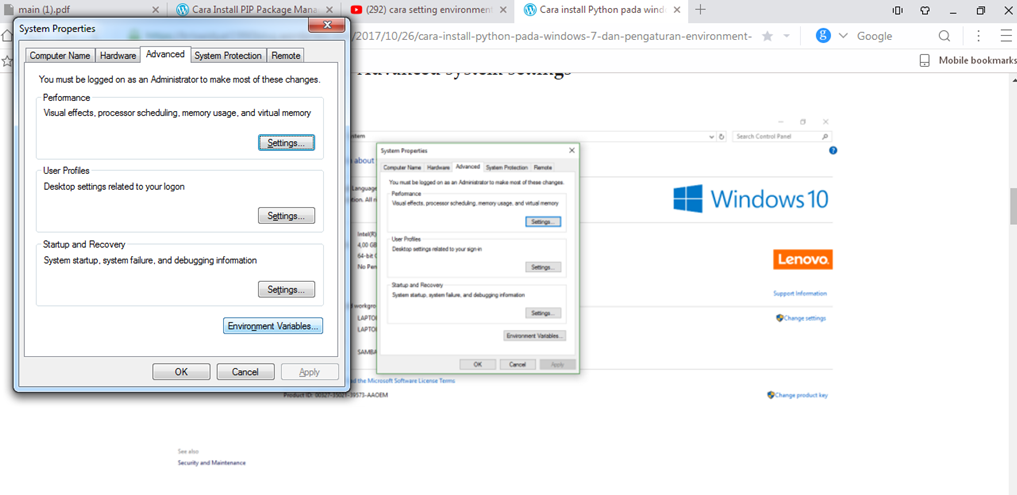
\includegraphics[scale=0.4]{src/soal3phyton2.PNG} 
\caption{gambar} 
\label{unhas} 
\end{center} 
\end{figure}

c.	Pada bagian system variables scrool sampai ketemu path dan klik lalu akan ada system edit

  \begin{figure}
\begin{center} 
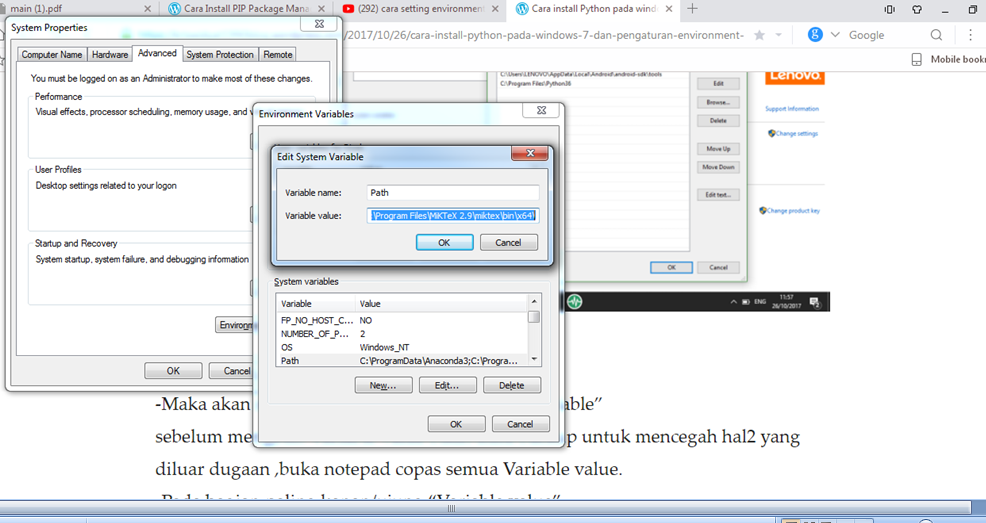
\includegraphics[scale=0.4]{src/soal3phyton3.PNG} 
\caption{gambar} 
\label{unhas} 
\end{center} 
\end{figure}

d.	Lalu sebelum di ubah di bagian variable value copy semua kata di dalam variable value dan di pindahkan ke notepad dan setelah itu di belakang directory tambahkan ;C: Python37 tergantung versi python kalian dan klik ok semuanya

  \begin{figure}
\begin{center} 
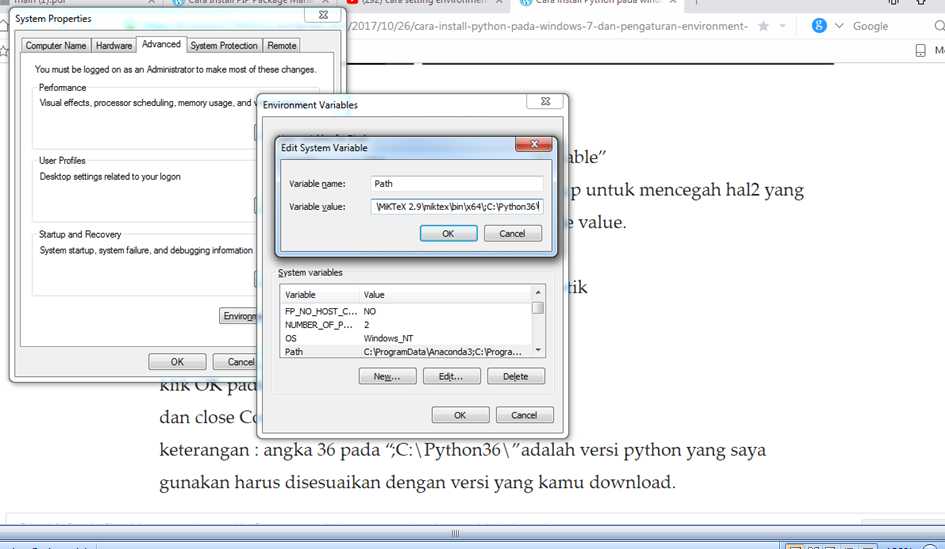
\includegraphics[scale=0.4]{src/soal3phyton4.PNG} 
\caption{gambar} 
\label{unhas} 
\end{center} 
\end{figure}

e.	Setelah di ok semua lalu buka cmd dan ketikan python dan akan muncul laman seperti ini

  \begin{figure}
\begin{center} 
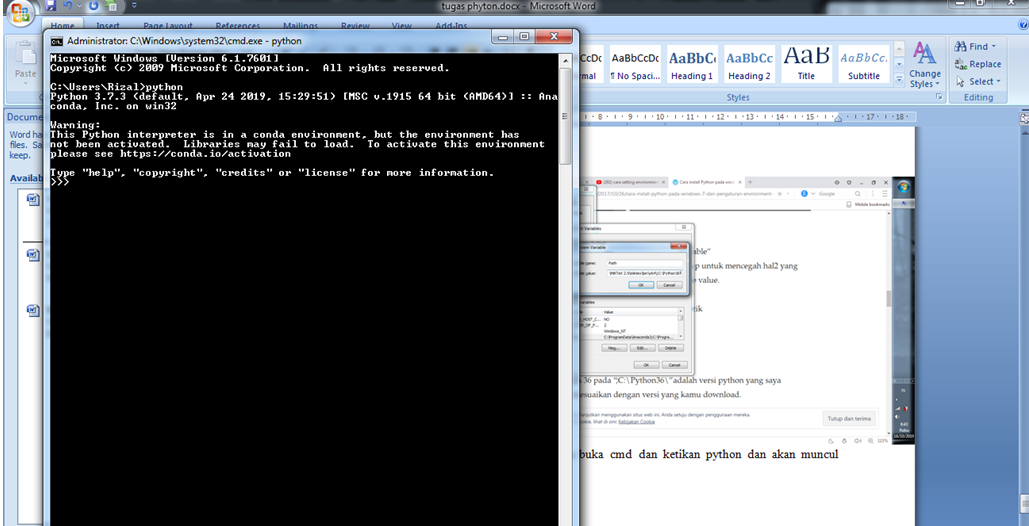
\includegraphics[scale=0.4]{src/soal3phyton5.PNG} 
\caption{gambar} 
\label{unhas} 
\end{center} 
\end{figure}

    
\item
mencoba entrepreter/cli melakui terminal atau cmd windows(5)

jawaban:
  \begin{figure}
\begin{center} 
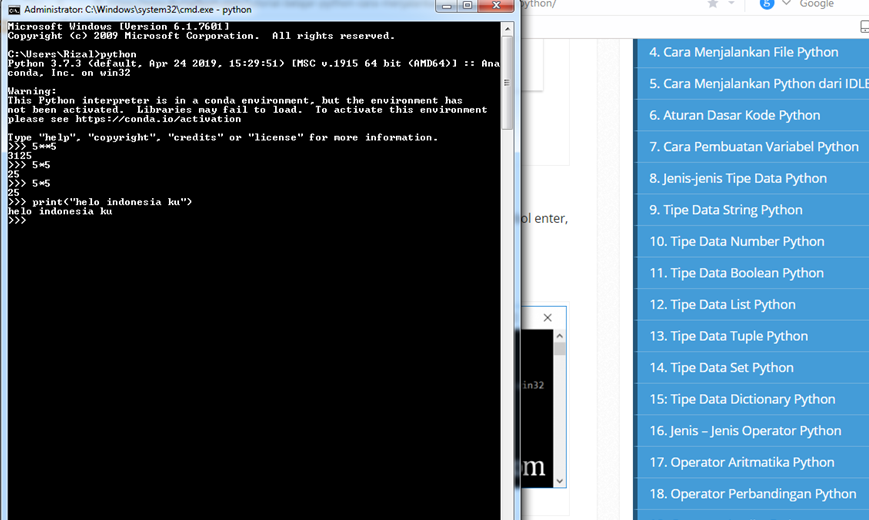
\includegraphics[scale=0.4]{src/soal4phyton1.PNG} 
\caption{gambar} 
\label{unhas} 
\end{center} 
\end{figure}
\item 
Menjalankan dan mengupdate anaconda dan spyder(5)
jawaban:
a.	Anaconda sudah di instal sebelumnya kita tinggal menjalankan nya
b.	Di cmd masukan conda install -c conda-forge basemap
Dan pastikan cmd terdapat pada dyrectory c:
\begin{figure}
\begin{center} 
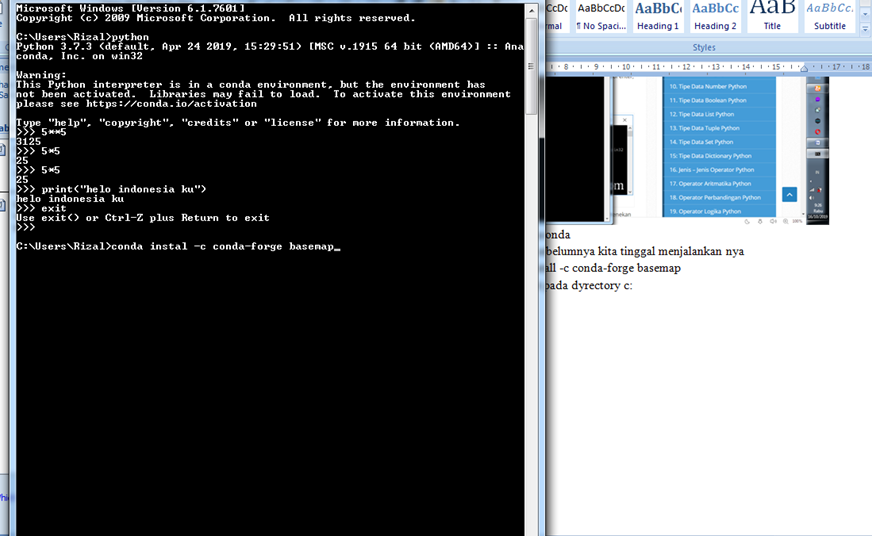
\includegraphics[scale=0.4]{src/soal5phyton1.PNG} 
\caption{gambar} 
\label{unhas} 
\end{center} 
\end{figure}

c.	Setelah instalasi selesai akan ada tulisan seperti dibawah
\begin{figure}
\begin{center} 
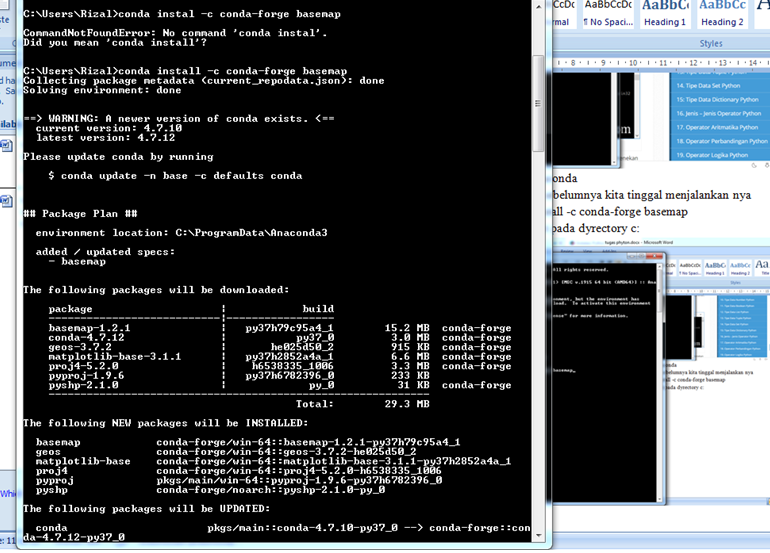
\includegraphics[scale=0.4]{src/soal5phyton2.PNG} 
\caption{gambar} 
\label{unhas} 
\end{center} 
\end{figure}

d.	Lalu setelah instalasi masuk lagi ke python di cmd

\begin{figure}
\begin{center} 
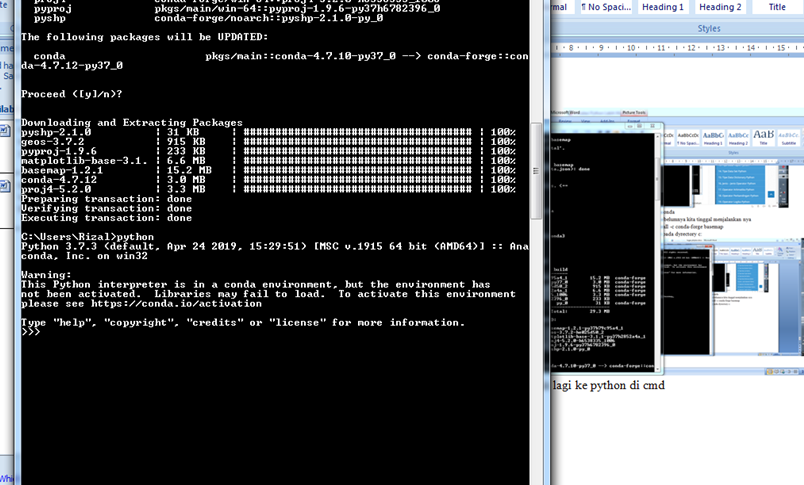
\includegraphics[scale=0.4]{src/soal5phyton3.PNG} 
\caption{gambar} 
\label{unhas} 
\end{center} 
\end{figure}

e.	Lalu coba import geopy di python apabila tidak ada berarti file tidak ada

\begin{figure}
\begin{center} 
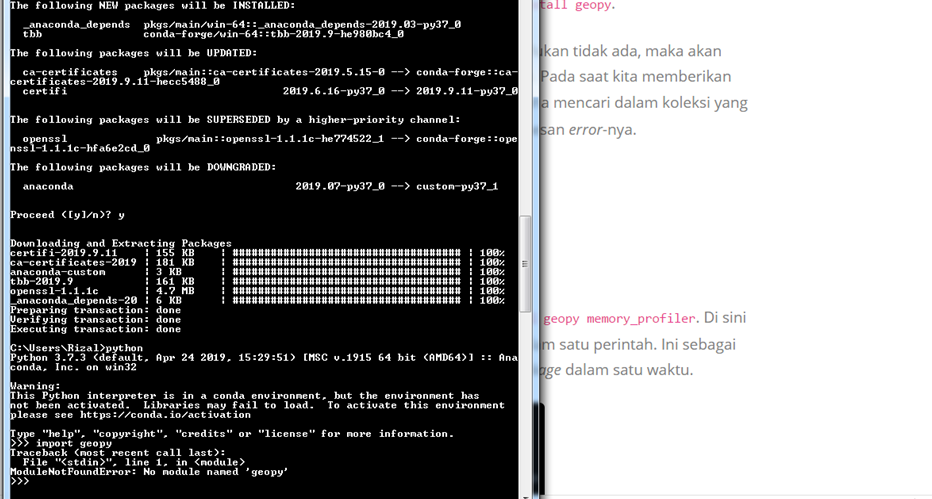
\includegraphics[scale=0.4]{src/soal5phyton4.PNG} 
\caption{gambar} 
\label{unhas} 
\end{center} 
\end{figure}

f.	pip install geopy memory profiler dibuat untuk mengatasi kendala yang ada diatas sampai proses nya beres

\begin{figure}
\begin{center} 
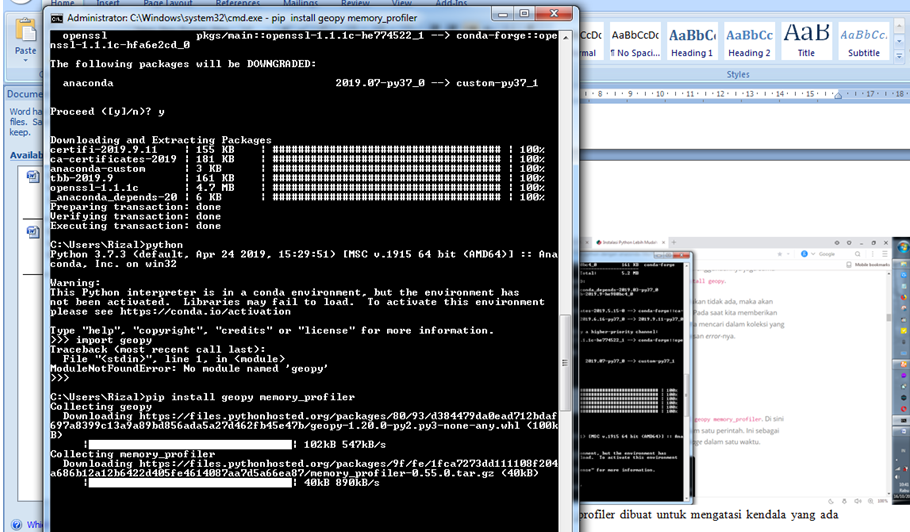
\includegraphics[scale=0.4]{src/soal5phyton5.PNG} 
\caption{gambar} 
\label{unhas} 
\end{center} 
\end{figure}

g.	setelah itu masuk lagi ke python import geopy geopy akan segera ter import

\begin{figure}
\begin{center} 
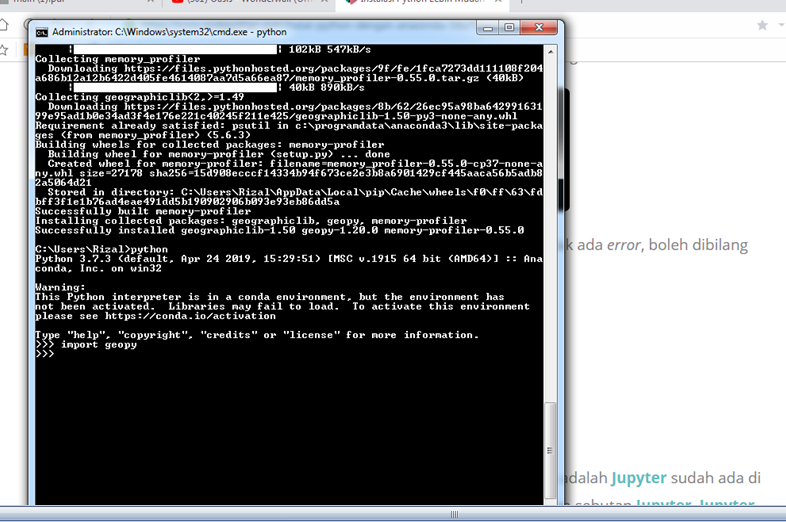
\includegraphics[scale=0.4]{src/soal5phyton6.PNG} 
\caption{gambar} 
\label{unhas} 
\end{center} 
\end{figure}

h.	Lalu buka aplikasi anaconda dan buka spider

\begin{figure}
\begin{center} 
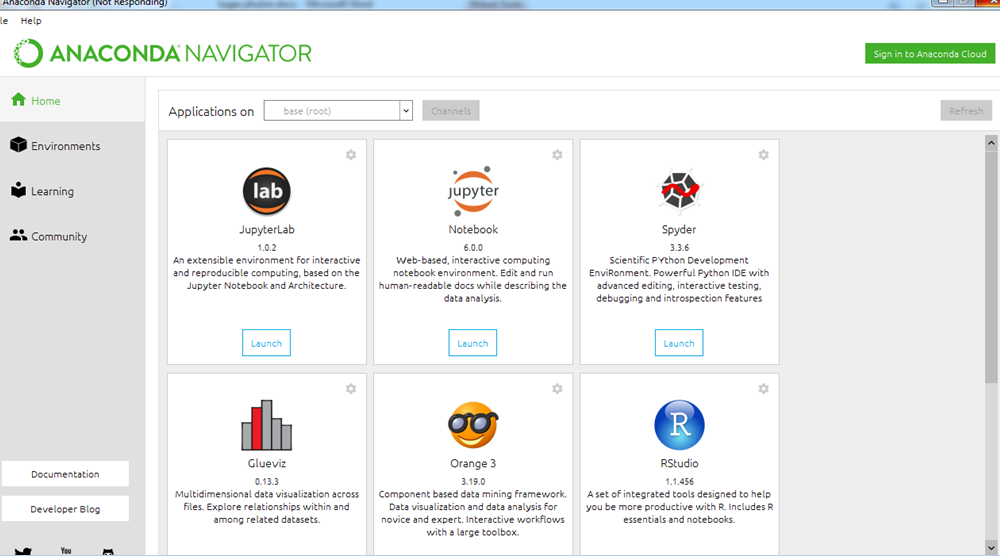
\includegraphics[scale=0.4]{src/soal5phyton7.PNG} 
\caption{gambar} 
\label{unhas} 
\end{center} 
\end{figure}

i.	Tampilan aplikasi spider

\begin{figure}
\begin{center} 
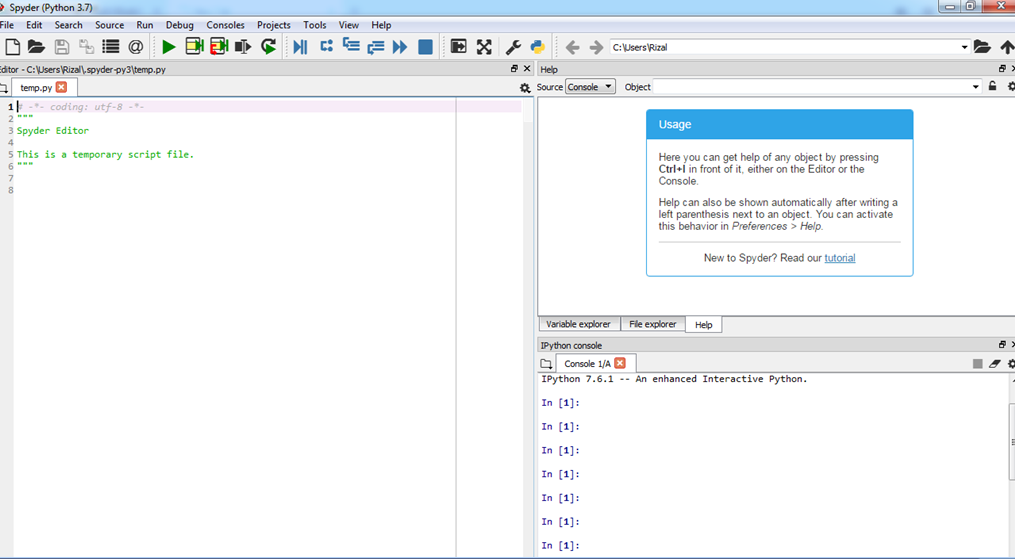
\includegraphics[scale=0.4]{src/soal5phyton8.PNG} 
\caption{gambar} 
\label{unhas} 
\end{center} 
\end{figure}

\item
Cara menjalankan Script hello word di spyder(5)
    
jawaban:
 \begin{figure}
\begin{center} 
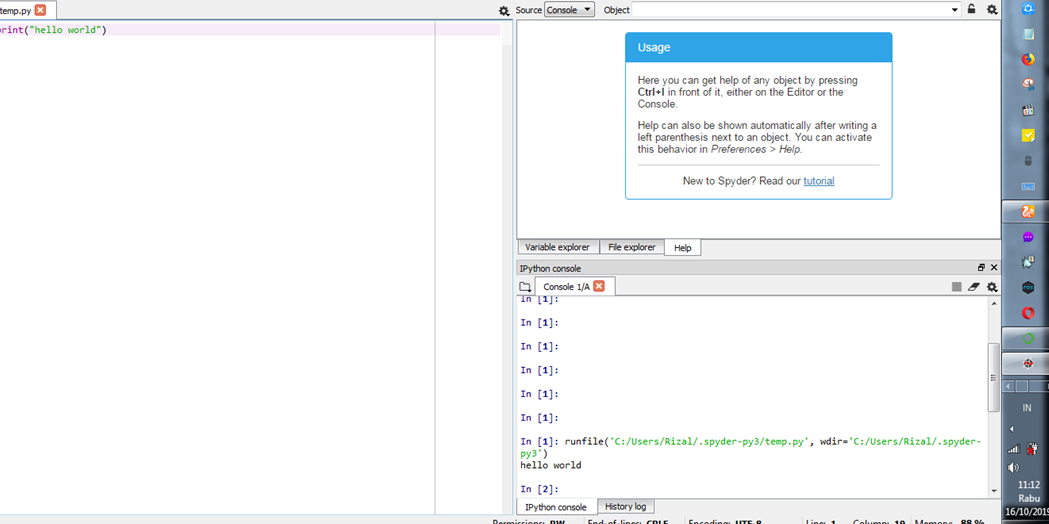
\includegraphics[scale=0.4]{src/soal6phyton1.PNG} 
\caption{gambar} 
\label{unhas} 
\end{center} 
\end{figure}   
    
\item
Cara menjalankan Script otomatis login aplikasi akademik dengan library selenium dan inputan user(5)


\item
Cara pemakaian variable explorer di spyder(5)

jawaban:
variable merupakan tempat penyimpan yang di gunakan untuk menyimpan data data dengan karakter karakter tertentu 

 \begin{figure}
\begin{center} 
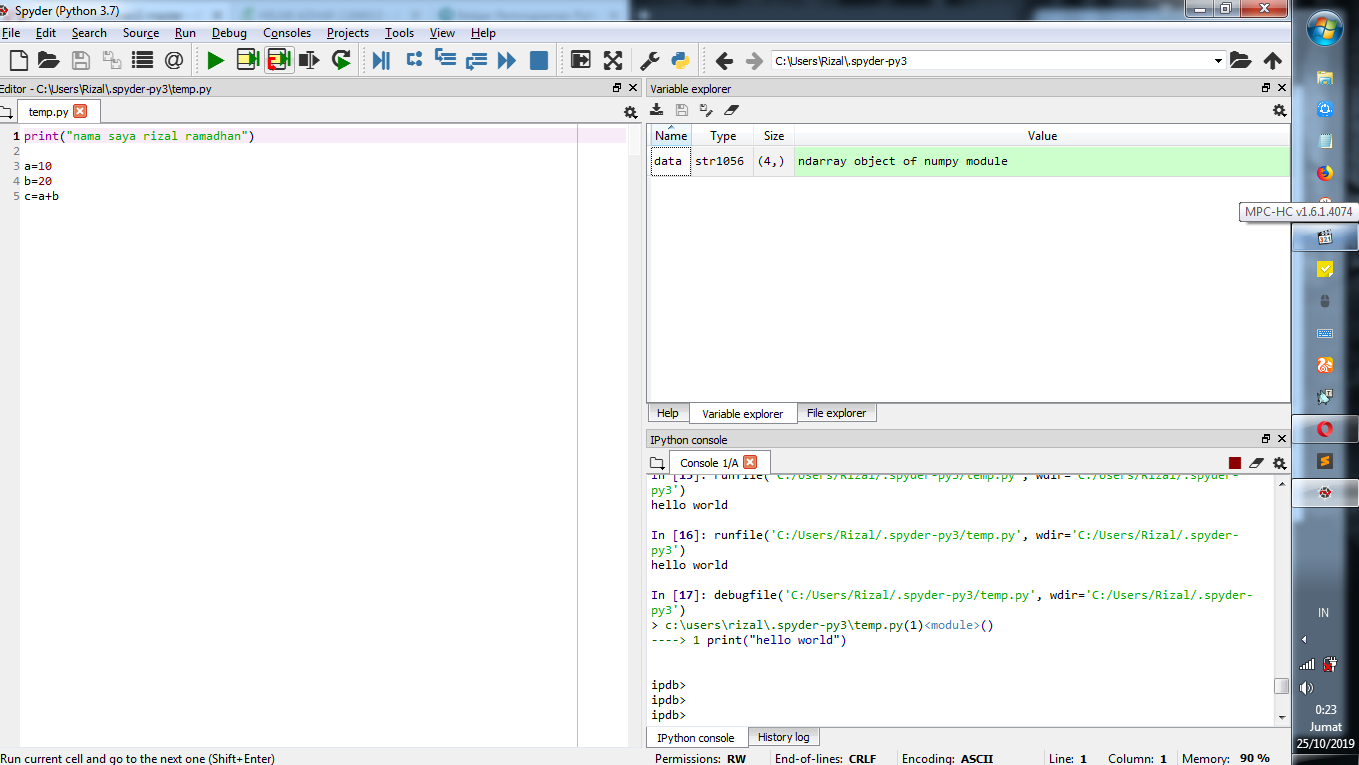
\includegraphics[scale=0.4]{src/baru.PNG}
\caption{gambar} 
\label{unhas} 
\end{center} 
\end{figure} 


\end{enumerate}


\section{Identasi}
Membuat file main.py dan mengisinya dengan script contoh python penggunaan selenium(minimal 20 baris) yang melibatkan inputan user, kemudian mencoba untuk mengatasi error identasi.
\begin{enumerate}
	\item
Penjelasan Identasi (10)
	\item
jenis jenis error identasi yang didapat(10)
\item
cara membaca error(10)
\item 
cara menangani errornya(10)
\end{enumerate}

\section{Presentasi Tugas}
Pada pertemuan ini, diadakan tiga penilaiain yaitu penilaian untuk tugas mingguan dengan nilai maksimal 100. Kemudian dalam satu minggu kedepan maksimal sebelum waktu mata kuliah. Ada presentasi kematerian dengan nilai presentasi yang terpisah masing-masing 100. Dan nilai terpisah untuk tutorial dari jawaban tugas di YouTube.Jadi ada tiga komponen penilaiain pada pertemuan ini yaitu :
\begin{enumerate}
	\item tugas minggu hari ini dan besok (maks 100). pada chapter ini
	\item presentasi csv (maks 100). Mempraktekkan kode python dan menjelaskan cara kerjanya.
	\item pembuatan video tutorial youtube tentang tutorial dari jawaban tugas.(nilai maks 100)
\end{enumerate}
Waktu presentasi pada jam kerja di IRC. Kriteria penilaian presentasi sangat sederhana, presenter akan ditanyai 20(10 pertanyaan program, 10 pertanyaan teori) pertanyaan tentang pemahamannya menggunakan python dan program agan dibuat error hingga presenter bisa menyelesaikan errornya. jika presenter tidak bisa menjawab satu pertanyaan asisten maka nilai nol. Jika semua pertanyaan bisa dijawab maka nilai 100. Presentasi bisa diulang apabila gagal, sampai bisa mendapatkan nilai 100 dalam waktu satu minggu kedepan.
